\documentclass [ngerman,a4paper,twoside,12pt,listof=totoc]{scrreprt} % lädt die Documentenklasse
\usepackage[ngerman] {babel}
\usepackage[utf8]{inputenc}
\usepackage[T1]{fontenc}
\usepackage{graphicx}
%\usepackage{titlesec}
\usepackage{longtable}
%\usepackage{amssymb}
\usepackage{wrapfig}
\usepackage[footnote]{acronym}
\usepackage{url} 
\usepackage{tocbibind}
\usepackage{hyperref} % Referenzieren 
\usepackage{multibib}
\usepackage{xcolor}%farbe
%\usepackage{longtable} % Merhspaltige Tabellen
\usepackage{amsmath} %Math

%glossar

\usepackage[numberedsection]{glossaries}
\makeglossaries
%Abkürzungen
\usepackage{acronym}







%Literaturverzeichnis 
\newcites{Refs,Urls}{Literaturverzeichnis,Verzeichnis der Webadressen}



\newcommand{\sectionbreak}{\clearpage}
\title{Praktikumsbericht}
\subtitle{Florian Häusler \\ InterMedCon GmbH}


\begin {document}
%\begin{titlepage}
%
%\end{titlepage}

\maketitle
\tableofcontents
%\include{Abkuerzungen}
\listoffigures% Abbildungsverzeichnis
%\listoftables% Tabellenverzeichnis
%\lstlistoflistings%Quellenverzeichnis


\chapter{Einleitung}
\section{Praktikumsbetrieb}
Bereits vor meinem Praktikumsbeginn hab ich vom 1. Dezember 2018 bis 31 Januar 2019 als Werksstudent bei der Intermedcon GmbH gearbeitet. Mir erschien der Zeitraum für ein Praktikum ziemlich kurz, ein neues Projekt im Dezember 2018 Startete und  im letzten Semester besuchte ich nur zwei Kurse.  Da hat es sich  angeboten als Werksstudent in das Team und das neue Projekt einzusteigen, um die Einarbeitung zu erleichtern. 

Die Intermedcon GmbH hat Standorte in Münster, Kiel und Berlin. Ein Großteil der Entwickler befindet sich in Berlin Dorotheenstraße, wo ich auch meinen Platz bekommen habe. Vor Ort ist auch der Technische Leiter zwei Webentwickler und ein  Android  Entwickler sowie Mitarbeiter von einem Tochterunternehmen. Den Mitarbeitern wurde es freigestellt ihre Arbeit auch im Home Office zu erledigen. Die Personalabteilung und Geschäftsführer befinden sich in Münster bzw. Kiel. 

Das Unternehmen hat sich spezialisiert auf  eHealth Anwendungen, Auftraggeber sind hierbei mit Privaten und Gesetzlichen Krankenkassen sowie Pharma-Unternehmen. Die Intermedcon GmbH ist hierbei in Zahlreiche öffentlichen Forschungs- und Förderprogrammen vertreten und arbeitet mit Zahlreichen internationalen Partnern zusammen u.a Dänemark, Schweden und Niederlande. Gerade für die Organisation und Aufbereiten von Medizineschen Studien werden neue Softwarelösungen benötigt, gerade in Internationalen Projekten.
%todo test entfernen
\gls{computer}
\ac{ts}




\chapter{Projekt}
\section{Projektbeschreibung iSpine}\label{beschreibung}
Beim iSpine-Projekt handelt es sich um ein von der Europäischen Union gefördertes Projekt, welches im Verbund mit den dänischen Partnern Sens Motion durchgeführt wurde. Es sollte eine intelligente Selbstüberwachung für eine effiziente ambulante Behandlung von ambulanter Rückschmerzen entwickelt werden. Dafür sollte von der Firma Sens Motion ein neuer Sensor entwickelt werden, der verschiedene Bewegungsarten erkennen kann. Weiter sollte eine App zur Motivation und Unterstützung eines aktiveren Lebens entwickelt werden, eine Anpassung für weiter Therapien und Krankheitsformen sollte gegeben sein. Die Sensoren sollen mittels Pflaster an den Oberschenkel angebracht werden, Sie sind für den einmaligen Gebrauch und min. 14 Tage wasserfest. Folgende  Bewegungsarten sollen durch den Sensor ermittelt werden können: Ruhend, Gehen, Laufen, Fahrradfahren, Anzahl der Schritte. 


Die ersten klinischen Tests bei unserem Partner in Kopenhagen waren für April 2019 geplant. Hierfür sollten 100 Patienten mit unspezifischen und chronischen Rückenschmerzen ausgesucht,  die jeweils in zwei Gruppen eingeteilt werden. Die eine Gruppe sollte den Sensor und die App erhalten und die zweite Gruppe nur den Sensor ohne die App.  Die Begleitung der Studie war für einen Zeitraum für 6 Wochen angelegt. Grobe Anforderungen an die App waren dabei:
Sie sollte möglichst leicht bedienbar sein, da auch gerade älter Patienten und Einwanderer die App bedienen sollen. Es sollte die Möglichkeit geben Daten wie Alter, Gewicht, Größe zu hinterlegen, um so später Rückschlüsse auf Erkrankungen zu erkennen. Daten die vom  Sens Motion Sensor ermittelt wurden, sollten in die App integriert werden und der Patient sollte zu diesen Daten Feedback erhalten. Das Aktivitätsniveau sollte er dabei selbst definieren können.


\section{Teammitglieder und deren Aufgaben}\label{team}
Beim iSpine Projekt handelt sich um die erst native Android-App die von der InterMedCon GmbH entwickelt wurde. Die Zusammenstellung des Teams erfolgte erst kurz vor dem Start des Projektes, im November. Die Projektführung wurde zum großen Teil von unserem technischen Leiter aus Berlin und wurde später durch eine wissenschaftliche Mitarbeiterin aus Kiel unterstützt. Des Weiteren waren zwei Werksstudenten /-in als Android Entwickler sowie eine Designerin für die Mockups eingestellt worden, die ihren Sitz nicht in Berlin hatten und ihre Arbeit im Homeoffice verrichteten. Ab Januar ist ein weiterer Android Entwickler, erst als Teilzeit und später als Vollzeitkraft zum Team in Berlin hinzugekommen. Wie unter \ref*{einleitung} Einleitung bereits erwähnt, habe ich erst als Werksstudent und ab Februar im Praktikum als Android-Entwickler das Team unterstützen dürfen. 

\section{Projektablauf}
\subsection{Beginn/Vorbereitung}\label{kapBegin}
Projektstart für die App-Entwicklung  war der 3.Dezember. Das Gesamtprojekt startete aber bereits weit vor diesem Datum, mit der Entwicklung des Sensors und der \ac{api} für den Zugriff auf die Daten, durch unsere dänischen Partner. Es wurden bereits Studien geplant und erste Auswertungen mit der Hilfe einer Web-App durchgeführt. Zielgruppen wurden analysiert und grobe Anforderungen spezifiziert.

Wie bereits oben erwähnt startete am 3. Dezember mit einer Kickoff Veranstaltung in Form einer Telefonkonferenz mit den dänischen Partnern und der Projektleitung die Entwicklung der App. Ich durfte auch an diesem Gespräch teilnehmen, hierbei wurde uns die Programmschnittstelle erläutert und Testzugänge eingerichtet.
Weiter wurden technische Anforderungen  und eine grobe Zeitplanung besprochen. Dabei war gerade aus unserer Position eine konkrete Aussage zu treffen sehr schwer. Da viele Faktoren unklar waren, wie zum Beispiel Personalstärke, Fähigkeiten und Funktionsweise der \ac{api} und Auswertung der Daten.
Hierbei wurde auch entschieden, dass wir nicht die Synchronisation des Sensors vornehmen, sondern dies durch eine bereits vorhandene App realisiert werden soll. Um durch den begrenzten Zeitraum bis zum Studienbeginn zu erleichtern. Ein erster Prototyp sollte bereits Mitte bis Ende Januar fertig sein und die erste Studie sollte dann Ende Februar beginnen.

Kurz darauf folgte die erst Telefonkonferenz zwischen dem in Kapitel \ref{team} beschrieben Entwickler-Team. Hierbei wurden die Inhalte der Telefonkonferenz mit den dänischen Partnern ausgewertet.
Weiterführend musste sich auf die einzusetzenden  Werkzeuge geeinigt werden, da das Team an mehreren Standorten ihre Arbeitete verrichtete.

Nachfolgend wurde die Arbeit mit folgenden Arbeitsmitteln unterstützt:
\begin{description}
	\item[Slack] zur Kommunikation innerhalb des Teams, als auch mit den Dänischen Partnern.
	\item[\gls{git}] als Versionsverwaltungssoftware, was das Arbeiten am selben Code sehr vereinfacht.
	\item[Taiga] als Projektmanagementsoftware zur agilen Softwareentwicklung. Später konnte hier auch ein Bug-Report eingerichtet werden, wo die Dänischen Partner Fehler hinterlegen konnten.
	\item[GoTo-Meeting] für die Wöchentlichen Sprints die als  Telefonkonferenzen durchgeführt wurden.
	\item[Android-Studio] Eine von Google und IntelliJ  basierende Entwicklungsumgebung.
\end{description}
 Es wurde sich auch auf eine wöchentliche Iteration geeinigt, wo jeder seine Arbeitsfortschritte und  Probleme im Arbeitsprozess vortragen  konnte.
 
\subsection{Durchführung}\label{durchführung}
Wie bereits erwähnt war unsere App abhängig von den Daten die wir von der API bekommen. Daher mussten einige Punkte im Vorfeld geprüft werden:
\begin{itemize}\label{stichpunkte}
	\item Wie erfolgt die Authentifizierung?
	\item Wie und wer legt neue Patienten an?
	\item Welche Daten stehen uns in der API zur Verfügung?
	\item Welche Daten brauchen wir?
	\item Welche Request müssen gesendet werden, um an die gewünschten Daten zu bekommen?
\end{itemize}
Hierbei kam es gerade in der Anfangszeit zu Problemen. Da es sich bei der API um eine Beta-Version handelte, weitere Änderungen vorgenommen wurden und die Verfügbarkeit eingeschränkt war.
Wir haben dafür eine kurze API Dokumentation bekommen und Testanfragen über \gls{postman} realisiert, um das Verhalten der API zu analysieren. Dabei war eine funktionierende Kommunikation mit den dänischen Partnern wichtig! 
Nachdem die Fragen geklärt waren, konnten erste Mockups und User Storys erstellt werden. In der APP-Entwicklung konnten dann die ersten Anmeldeseiten entwickelt werden. Außerdem wurden Bibliotheken recherchiert, die das Anfragen und Verarbeiten der Daten von der API erleichtern sollten.
% besser erklären warum!!
Die Betaversion der  API und neue Anforderungen machte ein lokales Zwischenspeichern der Daten unverzichtbar. So kam es zu Zeiträumen in der die API nicht erreichbar war, oder  es nach der Synchronisation des Sensors 10-20 min dauerte bis  Daten von der API geladen werden konnten.
Damit war das vorhergehende Speichermodell nicht mehr möglich/nötig und es musste auf eine lokale Datenbank umgestellt werden. Weitere Anforderungen wie eine
% live data mit ins glosar aufnehmen
 Hintergrundaktualisierung oder Notifikation machte den Einsatz von \gls{live}  (Observer) Notwendig. Dabei wurden  Daten die durch die API in der Datenbank verändert wurden,  in der aktuellen Ansicht aktualisiert. Es sollten auch eigene Daten mit Hilfe der API hochgeladen werden. Damit die Nutzer bei dem Wechsel ihres Gerätes nicht  ihre persönlichen Daten erneut eingeben müssen.
%tod Weiter Beschreibungen
\subsection{Abschluss}\label{abschluss}
Zwei bis drei Wochen vor dem Start der Studie, bekamen die Kliniker die App ausgehändigt um erste Tests durchzuführen. In einer wöchentlichen Telefonkonferenz wurden kleine Änderungen, Erweiterungen oder  Probleme besprochen. Die wie bereits beschrieben im Bug-Report festgehalten  und gegebenenfalls in die App intrigiert oder behoben wurden. Hierbei kam es auch  zur Anpassungen an der API, so dass der Anmeldeprozess umgestellt wurde, von Nutzernamen und Password auf Telefon und SMS/Pin. Durch den Einsatz der Bibliotheken war die Umstellung nicht so ein großes Problem wie erst vermutet. Es mussten nur wenige Klassen und UI-Elemente angepasst werden. Weiter musste getestet werden ob alle Notifiakations funktionieren, ob die Hintergrundsynchronisation mit der externen App funktioniert. Da die Studie in Dänemark durchgeführt wurde, mussten  alle UI-Elemente übersetzt und deren konkrete Übertragung getestet werden. In der Studie nutzten Probanden auch ihre eigenen Geräte, daher war es wichtig die App auch für verschiedene Displaygrößen auszurichten. Ein großer Teil der Studie nutzte allerdings bereitgestellte Smartphones, diese Geräte mussten beschafft konfiguriert und mit einer \ac{mdm}Software
ausgestattet werden. Damit spätere Updates oder Erweiterungen schneller eingespielt
%to bugs ins glossar
 werden können. Hierbei wurden alle erkannten \gls{bug}s erfolgreich behoben und die Studie konnte lediglich durch eine kurze Verzögerung durch die Lieferung der Smartphones gestartet werden. Während der Studienphase gab es weitere technische Gespräche mit den dänischen Partnern. Dabei kamen lediglich nur noch kleinere Fehler zum Vorschein, die schnell behoben werden konnten. Die Studie konnte dann erfolgreich starten, die Evaluation allerdings steht noch aus.

\section{Aufgaben am Projekt}
Wie in Kapitel \ref{kapBegin} beschrieben, durfte ich an der ersten Kickoff Veranstaltung mit den dänischen Partnern teilnehmen, um auch erste technische Fragen bezüglich der einzusetzenden API stellen zu können. Außerdem war es wichtig das dänische Team kennenzulernen, da die Umsetzung eine enge Zusammenarbeit voraussetzt. Dies war wichtig da ich nachfolgend im Team für die Datenbeschaffung über die API verantwortlich sein durfte.

Dabei war es erst mal notwendig den Request Ablauf der API herauszufinden, um die in Kapitel \ref{stichpunkte} gestellten Fragen beantworten zu können. Dies ging einerseits über eine kleine Webdokumentation und da nicht alle Endpunkt richtig beschrieben
% gloasar Postman anpassen
 waren über \gls{postman}. Hiermit konnte erstmals außerhalb der Anwendung das Verhalten der API analysiert werden, die gewünschten Request anfragen gefunden und die ersten Daten empfangen werden. Nachfolgend sollte ich eine Lösung finden, die Daten von der API in unsere App zu übermitteln. Hierbei hat sich die Bibliothek \gls{retrofit} sehr nützlich herausgestellt. Bei \gls{retrofit} werden die Anfragen in einem Interface beschrieben wie Header, Anfrage (POST, GET), Response Objekt , Request
 % baut ist zu umgangssprachlich
  Objekte und Endpunkt der API. Retrofit setzt mit der Hilfe der Basisadresse die Anfrage zusammen und liefert die Antwort wieder zurück. Diese Request und Response Objekte werden als \ac{pojo} Objekte beschrieben und die Bibliothek kümmert sich um die richtige Serialisierung. Ein manuelles Parsen der JSON Objekte ist somit nicht mehr notwendig, dies hat sich gerade bei Umstellungen der API Anfragen oder bei Veränderungen von Objekten vorteilhaft erwiesen.

%t besser beschreiben warum nicht zuverlässig ggf vewweis oben
Da sich die API wie in \ref{durchführung} beschrieben im Verlauf des Projektes als nicht zuverlässig herausgestellte  und wir zum Vorantreiben und testen der UI-Elemente sowie der weiteren Logik auf Daten angewiesen waren, haben wir uns für ein Caching der Daten entschieden. Ich durfte mir darüber Gedanken machen und wir entschieden uns für   die \gls{room} Bibliothek. Es handelt sich dabei um eine Relationale Datenbank, dabei konnte man die von der API bereits verwendeten \ac{pojo} Objekte für das \ac{orm} wiederverwenden. Die Bibliothek macht den Zugriff auf die Datenbank einfach über ein \ac{dao}  möglich und übernimmt ebenfalls das \ac{or}-Mapping. Der Einsatz von Room erleichterte die Programmierung, auch durch den Einsatz von Konvertern. Die es ermöglichten nicht primitive Datentypen zu Speichern . 
%t beschreiben was vorher vorhanden war
Durch den Umstieg auf die Room Datenbank wurde das vorhandene Speicherkonzept verworfen und die Funktionen in die neue Datenbankstruktur migriert.
Vorher haben wir unsere Daten in \gls{sharedpreferences} für die dauerhafte Speicherung und während der Laufzeit auf das Singleton-Muster gesetzt.
Ein ER-Modell der Datenbank befindet sich  als Abbildung:\ref{fig:ER-Modell}  im Anhang.
%Da nicht mit einem so umfangreichen Speicherung von Daten gerechnet wurde, existierte bereits eine SQL-Lite Datenbank, in der Persönliche Daten und andere Werte hinterlegt wurden. Um nicht mehrgleisig zu fahren wurden diese Daten in die Room-Datenbank integriert.%todo erstellen eines ERM und erstellen eines kleinen Klassen Diagramms zugriff auf API und Room Datenbank

Wie in \ref{abschluss} beschrieben kamen es durch Veränderungen an der API noch zu weiteren Anpassungen innerhalb unserer App. So wie oben erwähnt sollte der Authentifizierungsprozess geändert werden, es sollten eigene Metadaten gesendet und verarbeitet werden. Wir haben weitere Metadaten erhalten, die einen Feedback Zeitraum beinhalteten. So konnte die in \ref{beschreibung} beschriebene Feedback Periode hinzugefügt und die persönlichen Daten auf dem Server gespeichert werden.
%Da sich die \ac{api} noch in einer Beta Version befand kam es noch zu Veränderungen, auf die wir im Entwicklungsprozess reagieren mussten. So wurde der Authentifizierungsprozess mit Anmeldenamen + Passwort auf Telefonnummer + SMS/Pin umgestellt. Weiter sollten Metadaten auf dem Server gespeichert werden oder es sollte ermöglicht werden den Patienten eine Feedback-Zeitraum zuordnen zu können. In dem er seine Bewegungsdaten sehen kann ansonsten sind  Sie verborgen.


Weitere Anforderungen und der Einsatz von Hintergrundaktualisierungen machten wiederum Veränderungen notwendig. Hierbei durfte ich mich mit dem Einsatz von LiveData beschäftigen. LiveData ist ein Observer-Muster, es ermöglichte  LifeCycle Konflikte zu verhindern und das Zusammenspiel zwischen API und Room-Datenbank zu verbessern. Da man die Tabellen einer Datenbank direkt als Observable Objekt deklarieren kann, werden Veränderungen die durch die  API hervorgerufen werden, direkt  an die aktuelle View weitergegeben.

Zum Ende des Projektes durfte ich  noch bei Frontend Arbeiten unterstützen. Dabei ging es hauptsächlich um responsive Anpassungen zwischen den verschiedenen Display Größen(Smartphone,Tablet), kleinere Fehlerbehebungen und das Implementieren weiterer Fitnessübungen in Form von Bildern (Siehe Abbildung: \ref{fig:Fitnesübung}).
Final wurden Smartphones beschafft, die installiert, konfiguriert und versendet werden mussten. Dies Stellte den Abschluss des Projektes da.



% Einarbeitung in die Api

% lokales speichern von deaten da Api  unzuverlässige 

% darusfolgende einrichtung einer lokalen relationalen Datenbank

%  später änderungen an der Api (LogIn prozess) metadaten hochladen feedbachtime

% weiter anforderungen machte liveData notwendig . Gerade im zusammenspiel Datenbank und Api

% Anpassungen an Tablet 
\chapter{Bezug zum Studium}
test
% todo Projektmanagement

%todo Realtionale Datenbanken

%todo Verteilte systeme 

%todo Mobile Anwendungen Android Studio und ios 

%todo arbeiten in gruppen 







%todo verstehen lesen von fremden code 
%todo nutzen aussagekräftiger klassennamen, variablen und methoden
%todo frühzeitige kommunikation 

\chapter{Ausblick}
\chapter{Anhang}
\section{ER-Modell}
\begin{figure}[ht]
	\centering
	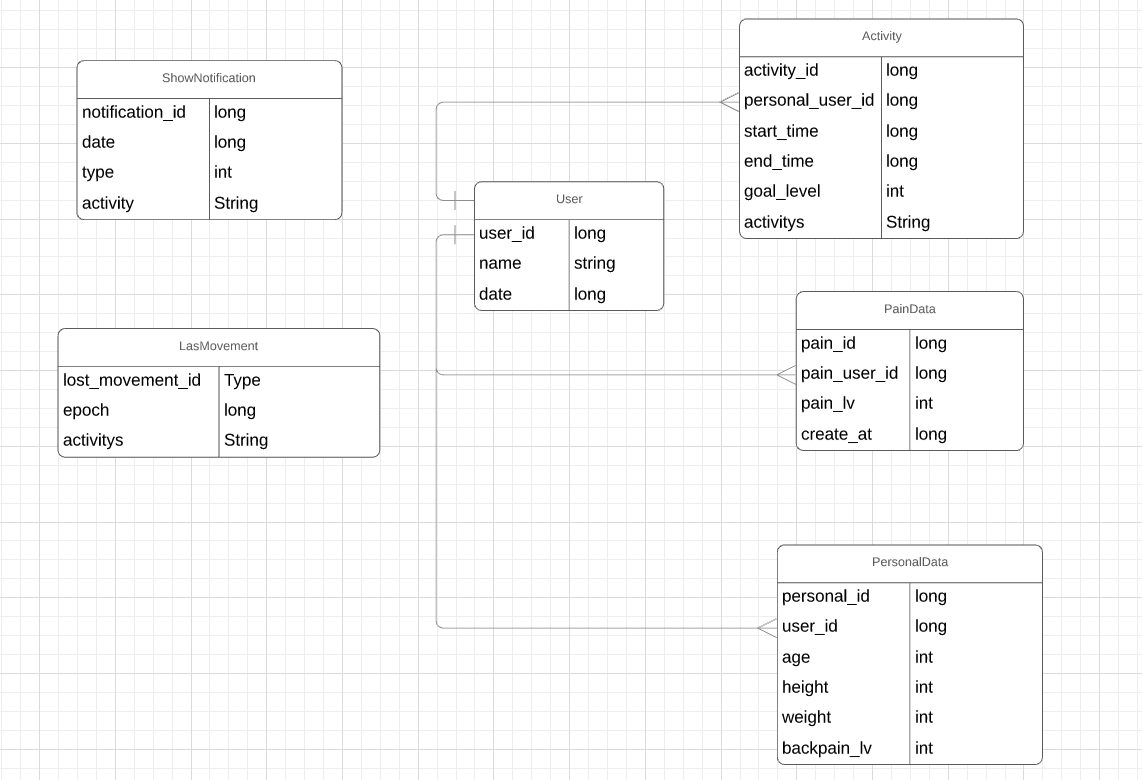
\includegraphics[width=1.1\textwidth]{Datenbank.png}
	\caption{\label{fig:ER-Modell}Grobes Datenbankmodell}
	
\end{figure}
\newpage

\section{Abbildungen}
\begin{figure}[ht]
	\centering
	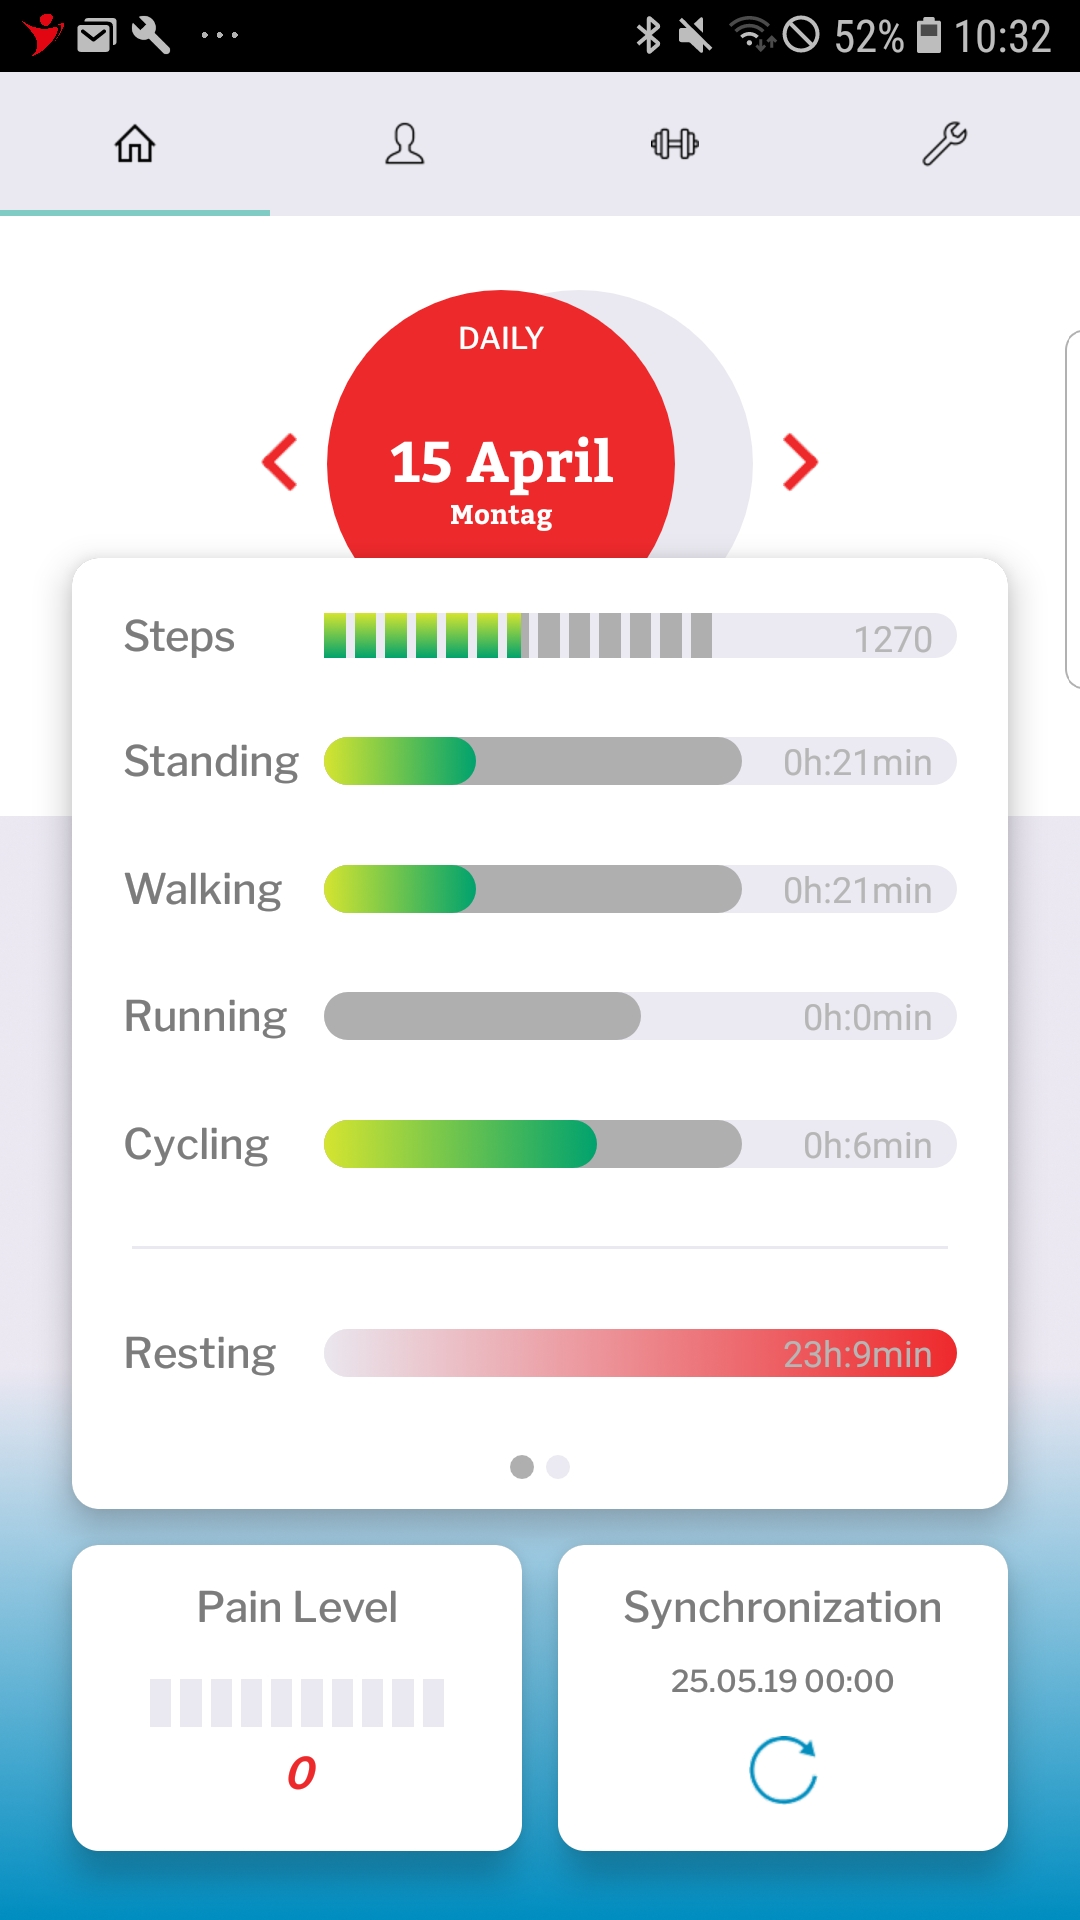
\includegraphics[width=0.5\textwidth]{Activitys.jpg}
	\caption{\label{fig:Activity}Aktivitäten mit den Daten von der API }
	
\end{figure}

\begin{figure}[ht]
	\centering
	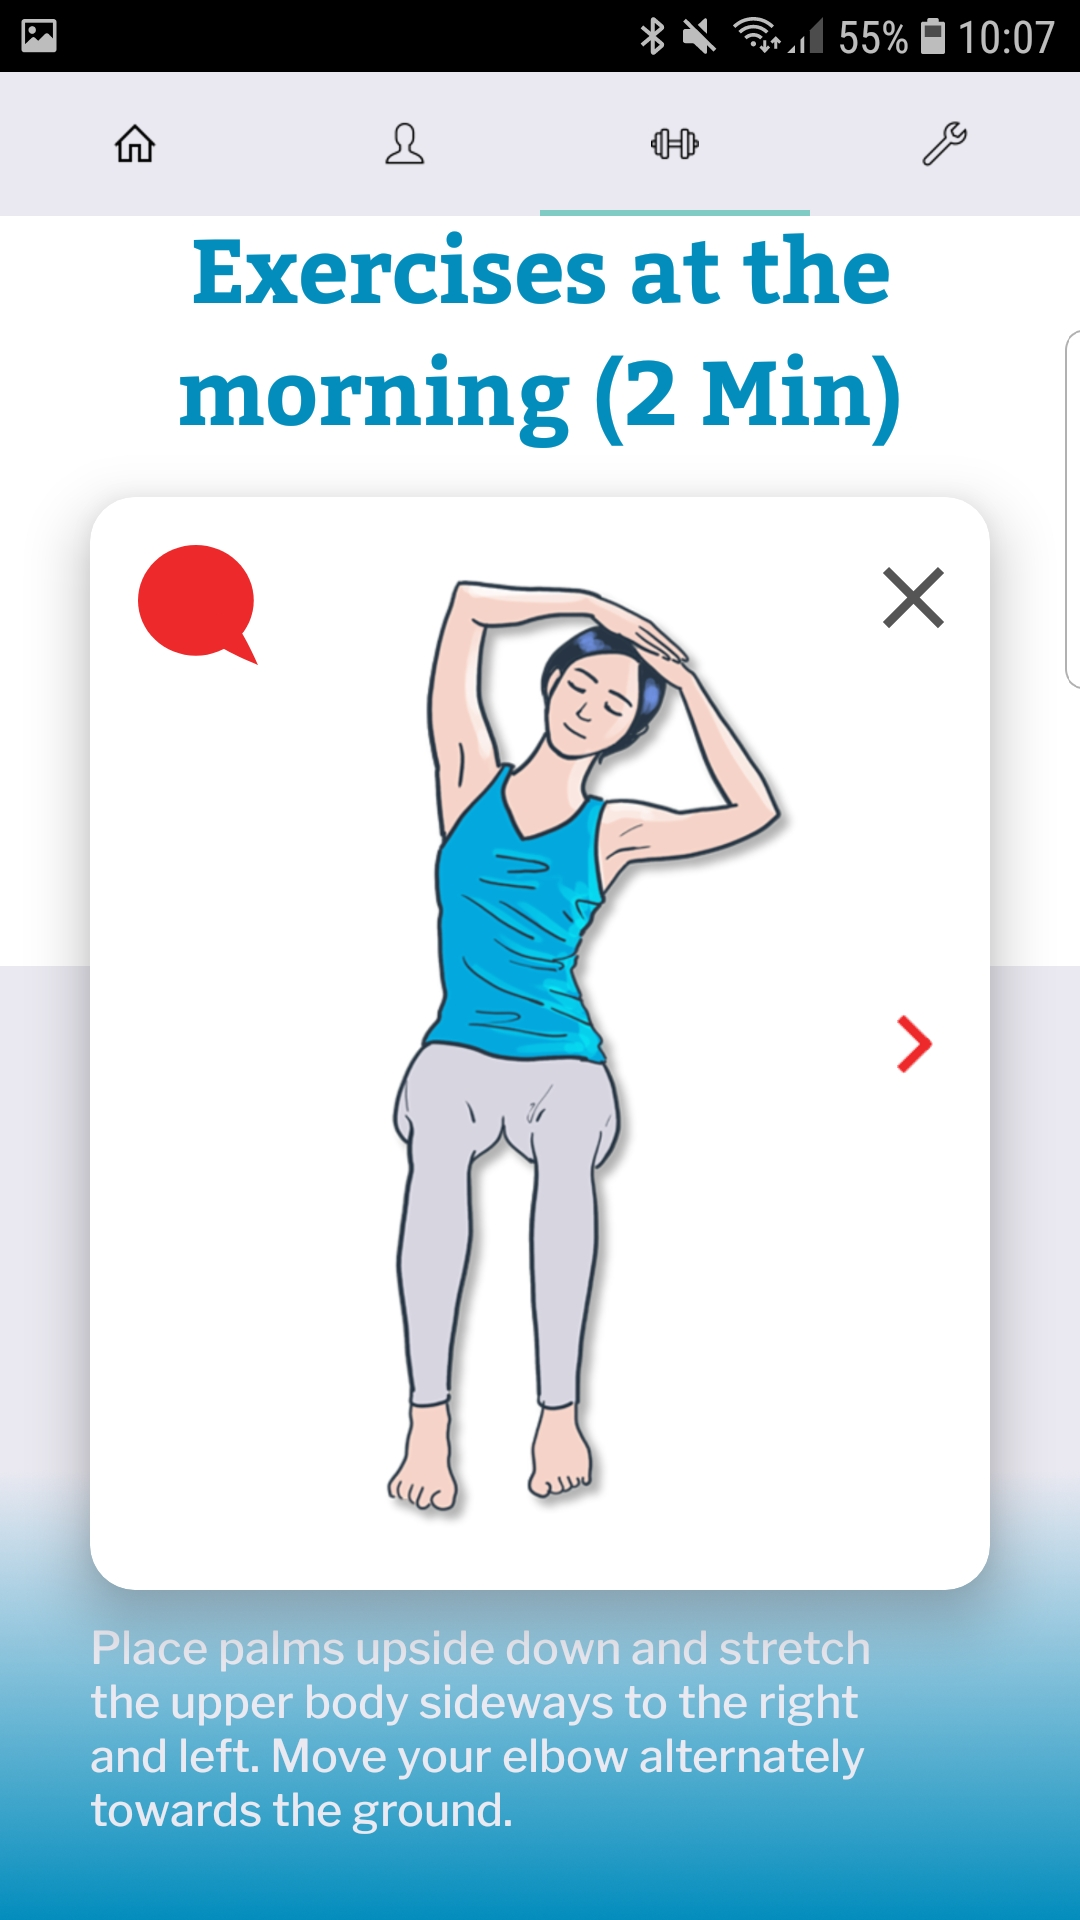
\includegraphics[width=0.5\textwidth]{excercise.jpg}
	\caption{\label{fig:Fitnesübung}Fitnessübungen zu einem bestimmten Schmerzbereich}
	
\end{figure}

\begin{figure}[ht]
	\centering
	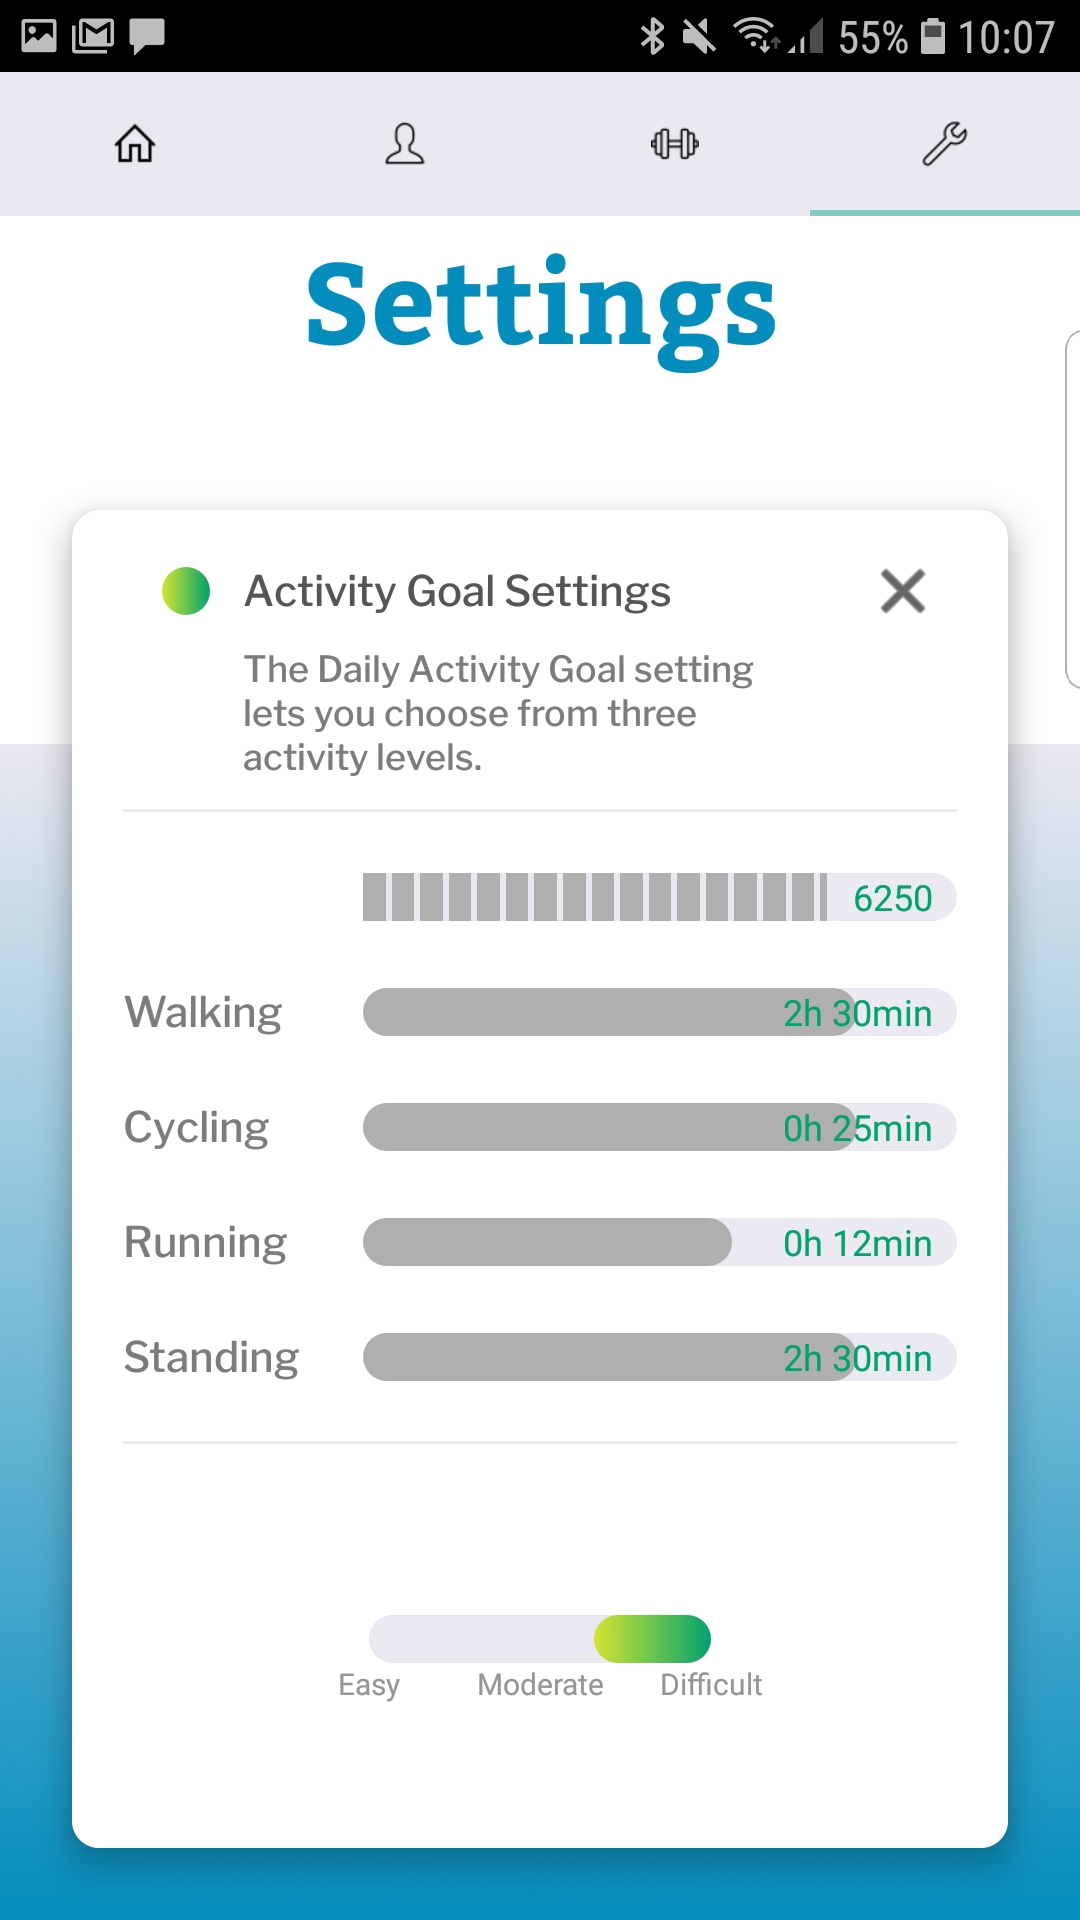
\includegraphics[width=0.5\textwidth]{settings.jpg}
	\caption{\label{fig:GoalSettings}Einstellung der Schwierigkeitslevels}
	
\end{figure}


\newglossaryentry{computer}
{
  name=computer,
  description={is a programmable machine that receives input,
               stores and manipulates data, and provides
               output in a useful format}
}
\newglossaryentry{datenagnostisch}
{
	name=datenagnostisch,
	description={Daten unspezifische Übertragung}
}
\newacronym[description={Modulare Bauweise}]{mbw}{MBW}{modulare Bauweise}





%\bibliography{LoRa}
%\bibliographystyle{plain}
%old
\printglossary[title=Glossar] % Glossar
\newpage
\vspace*{\fill} 
\begin{tabular}{ccccccccc}
	&   &   &  & & & & & \\\cline{1-2}\cline{4-4} \cline{6-7} \cline{9-9}
	
	& Ort, Datum & & Unterschrift && Ort, Datum & & & Unterschrift  \\
	&					&&	Praktikant	&&						&&& Praktikumsbetrieb
	
\end{tabular}









%\bibliographystyleUrls{plain}
%\bibliographyUrls{BibliographyUrls}
\end{document}